A network is laid out on a grid of $n \times m$ cells. Each cell is either empty or holds a junction. A junction has openings in two, three, or four of the four cardinal directions --- up, right, down, left. A junction with exactly one opening never occurs: the pressure would burst it.

Two junctions in orthogonally adjacent cells are \emph{connected} if and only if both have openings facing each other. A \emph{loop} is a route that starts at some junction, moves along connections, and returns to the starting junction without using any connection twice.

The network is measured by the number of \emph{independent loops}$^{\dagger}$ it contains.

Each cell is described by a single integer $g_{i,j}$: $0$ for an empty cell, and otherwise the sum of $1$ for an opening facing up, $2$ for right, $4$ for down, and $8$ for left. For instance, a junction whose openings face up and right is written as $g_{i,j} = 1 + 2 = 3$:

\begin{center}
  \def \htmlPixelsInCm {45}
  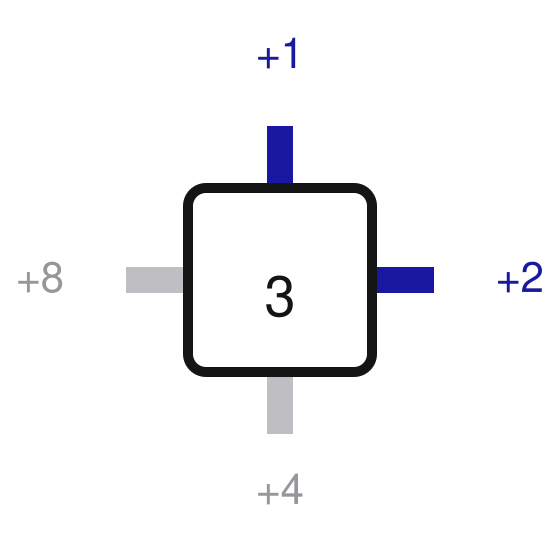
\includegraphics[width=3cm]{pipe-bits.svg}
\end{center}

Openings facing outside the grid connect to nothing.

The junctions are destroyed one by one: the whole sequence of $q$ destructions is given in advance; every destruction hits a cell containing a working junction, and no cell is hit twice.

After each destruction, report the number of independent loops remaining in the network.

{\small $^{\dagger}$ Formally, the \emph{number of independent loops} of the network is the largest $t$ for which one can choose a sequence of loops $L_1, L_2, \ldots, L_t$ such that every loop $L_i$ passes through at least one connection that none of the earlier loops $L_1, L_2, \ldots, L_{i-1}$ pass through.}
